\chapter{Presence of masked Modules at the ATLAS Detector}%\label{make}

\section{Overview of the ATLAS Detector}

In this section there will be given a short description of the structure of the ATLAS detector with a focus on the hadronic calorimeter system.
The ATLAS detector is a general purpose detector for high energy proton-proton collisions which is build up at the Large Hadron Collider (LHC) at CERN.
The LHC is a particle accelerator colliding protons with center of mass energies of currently \SI{13}{\tera\electronvolt} in RunII.
The overall structure of the ATLAS detector is cylinder symmetric around the beam axis and is build up in different layers from the inside to the outside.
The angle transverse to the beam axis is described as the azimuthal angle $\phi$ whereas the angle along the beam axis is described as the pseudorapidity $\eta$.
An overall cut-away view of the ATLAS detector is shown in figure \ref{ATLAS}.
\begin{figure}[H]
	\centering
	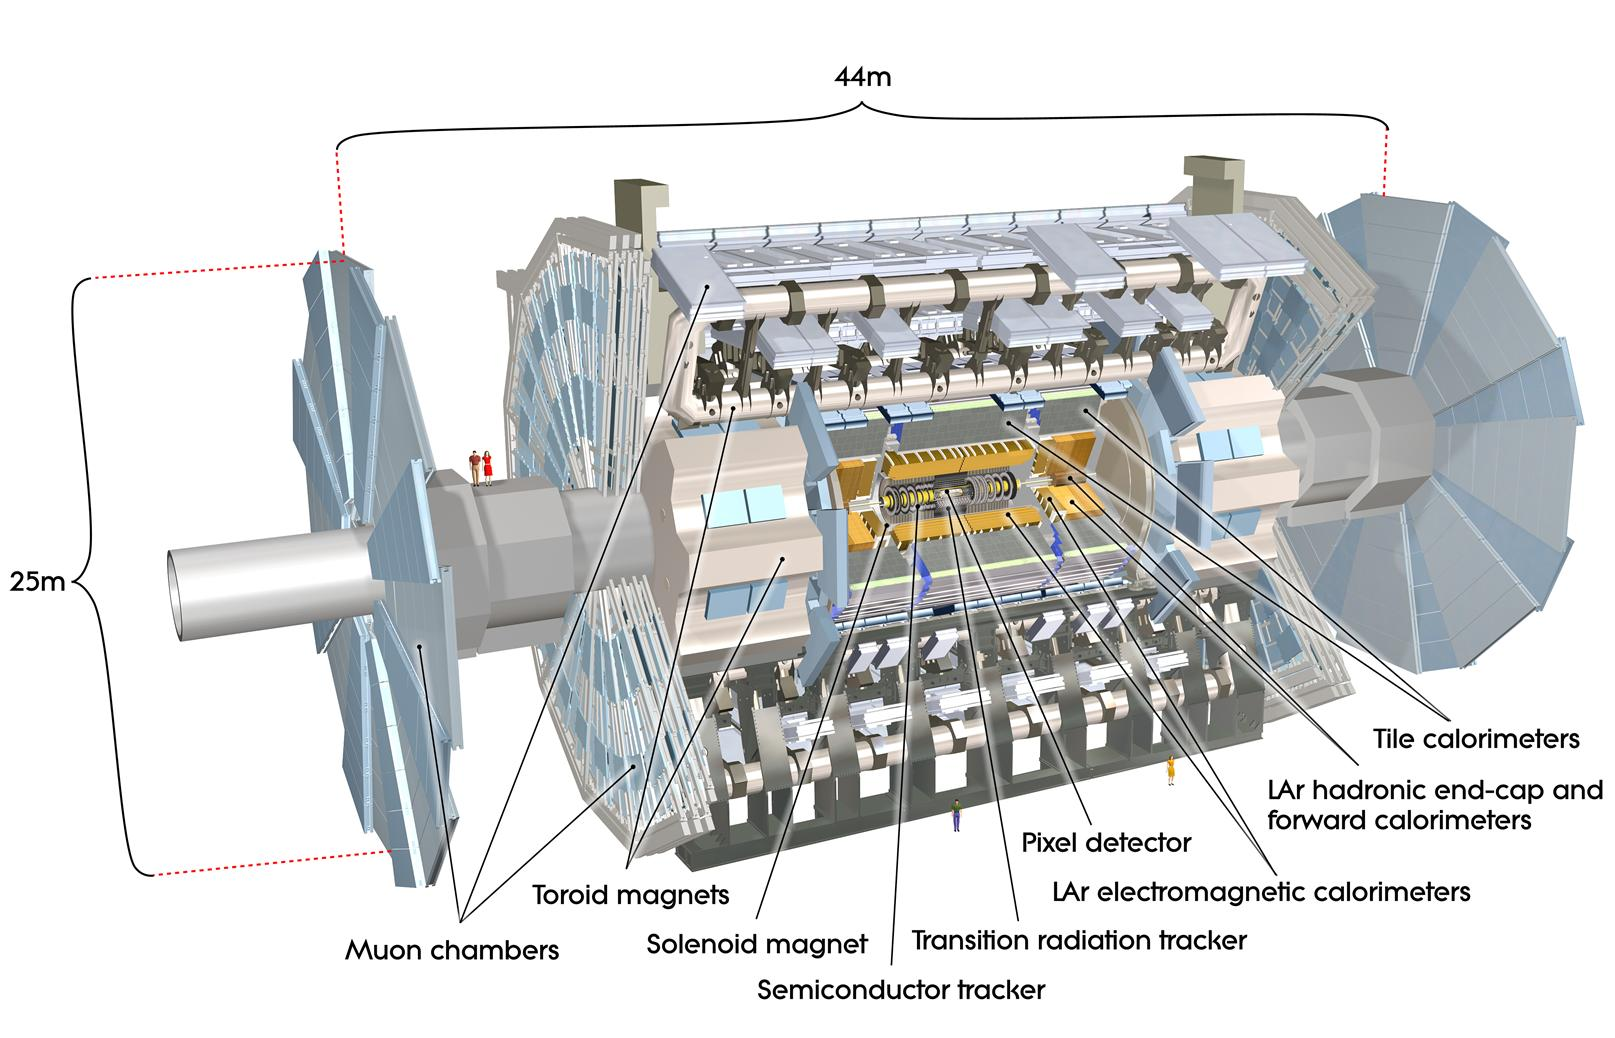
\includegraphics[width=\textwidth]{./Plots/figures_AtlasDetectorLabelled.png}
	\caption{Cut-away view of the ATLAS detector as detailed computer graphic.\cite{Aad:2008zzm}}
	\label{ATLAS}
\end{figure}
\subsection{The Inner Detector}
The innermost layer of the ATLAS detector is the Inner Detector (ID).
It is build by layers of silicon pixel and stripe detectors for precise measurements of particle tracks origin from the collision point.
The ID is permeated by a \SI{2}{\tesla} magnetic field for bending the charged particles track.
The track bending can be used for precise measurements of the momentum of charged particles.
In Addition the innermost layers of the ID can be used for vertex reconstruction.
The pixel and stripe detector systems cover in total a region of $|\eta| < 2.5$.
\subsection{Calorimeter Systems}
The calorimeter system of the ATLAS detector is build up in two layers and is designed to measure the energy deposits of hadronic and electromagnetic particles.
A cut-away view of the ATLAS calorimeter system is given in figure \ref{Calo}.
\begin{figure}[H]
	\centering
	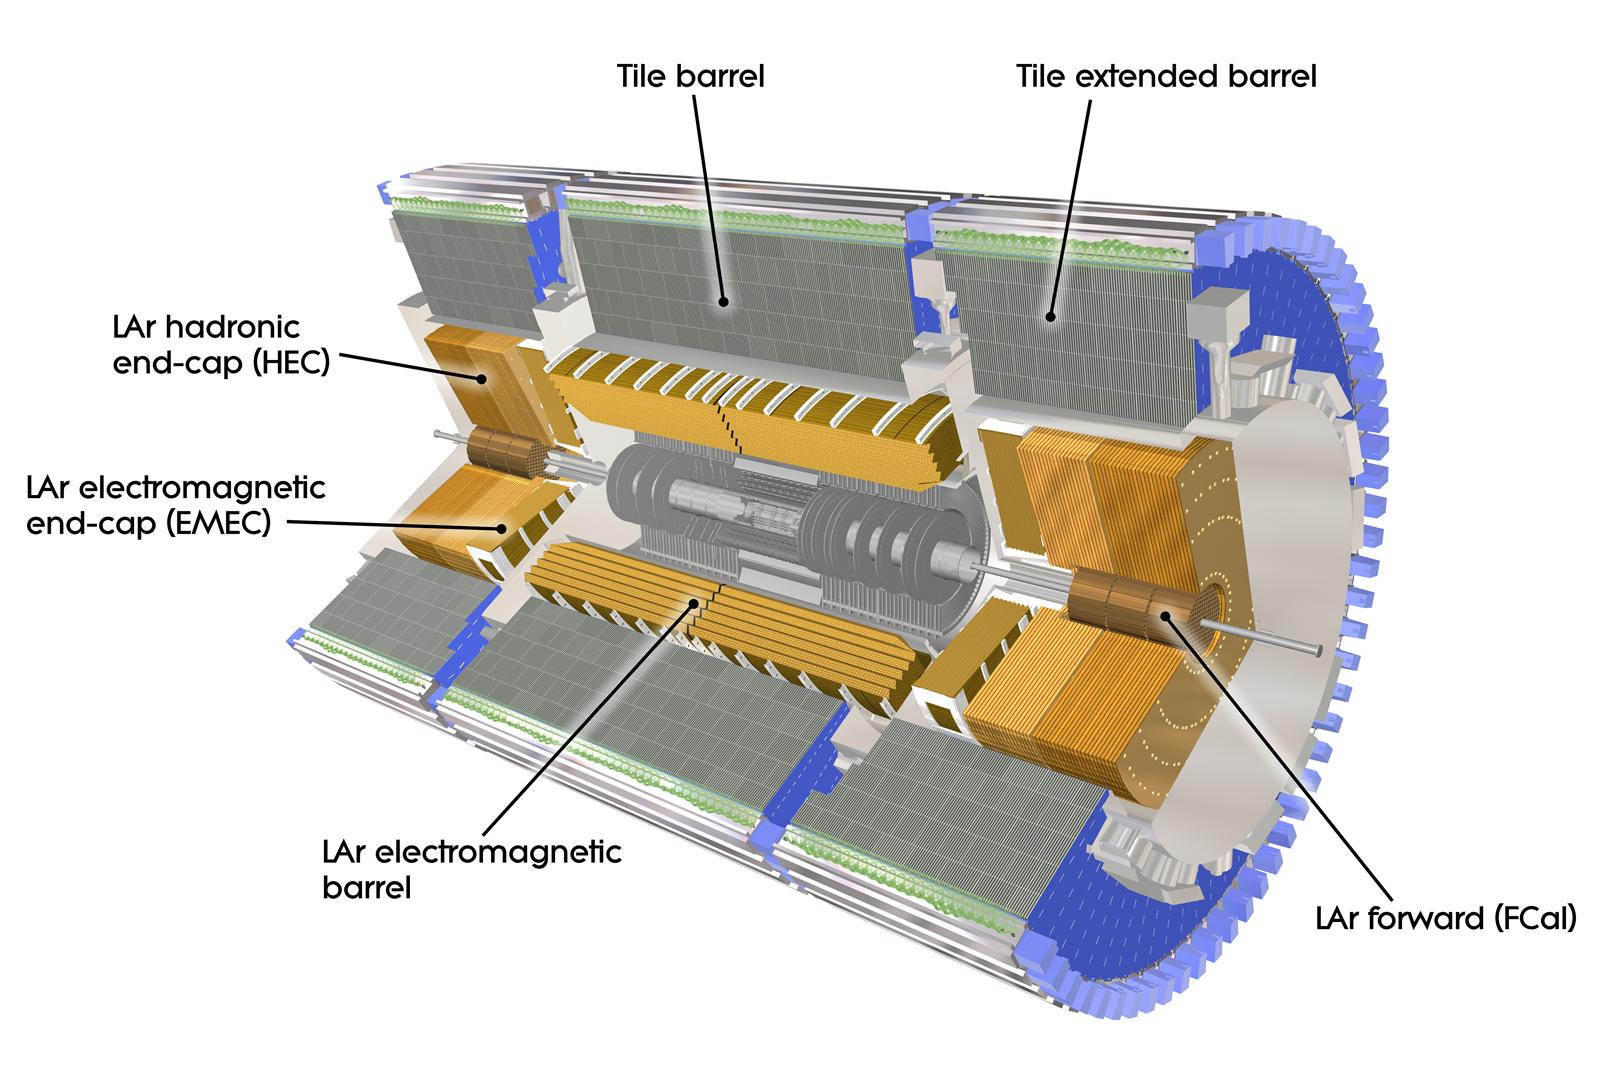
\includegraphics[width=\textwidth]{./Plots/atlas-calo-high.jpg}
	\caption{Cut-away view of the ATLAS calorimeter systems as detailed computer graphic.\cite{Aad:2008zzm}}
	\label{Calo}
\end{figure}
The inner layer of the calorimetry system is the liquid-argon electromagnetic calorimeter which covers in total a range of $|\eta| < 3.2$.
It is designed to absorb and measure most of the energy deposed by incoming electrons and photons but also detects energy depositions of hadronic particles.
The second layer of the calorimetry system is the hadronic calorimeter which is separated into a central barrel covering $|\eta| < 1$ and two extended barrels on the left and on the right of the detector covering each $0.8 < |\eta| < 1.7$.
The hadronic calorimeter is build as a sampling calorimeter and is constructed in layers of steel for energy absorption and scintillating material to measure the deposits.
Both electromagnetic and hadronic calorimeters also include forward calorimeters covering out wide regions in $|\eta|$.

As it is important for the following analysis, the specific segmentation of the hadronic calorimeter will be described here further.
The central barrel of the hadronic calorimeter is divided into two so called partitions LBA and LBC.
The LBC partition covers a region of $-1 < \eta < 0$ and the LBA partition covers $0 < \eta < 1$.
The extended barrels are each partitions called EBC and EBA, where EBC covers $-1.7 < \eta < -0.8$ and EBA $0.8 < \eta < 1.7$.
Each of this partitions is segmented into 64 modules in $\phi$, so that each module covers approximately a $\phi$ region of 0.1.
So the modules in the EBC for example are enumerated as EBC01 - EBC64.
\subsection{Myon System}
The outermost part of the ATLAS detector is the myon sytem for reconstruction of myon tracks.
Like the ID the myon system is permeated by a magnetic field to bend the tracks of the myons passing the detector.
\section{Jet and $\boldmath E_{\mathrm{T}}^{\mathrm{miss}}\unboldmath$ Reconstruction}
In proton-proton collisions various processes between elementary particles take place.
In many of this processes there are origin collimated "beams" of hadronic particles.
Those processes are called hadronisation processes and can be described with the strong interaction.
These "beams" are so called jets which are reconstructed as extended objects defined by their central axis position in the $\eta$-$\phi$-plane, their transverse momentum $p_{\text{T}}$ and their radius $\Delta R = \sqrt{\Delta\phi^2 + \Delta\eta^2}$.
So a jet can be characterised by specifying its four momentum and its $\Delta R$.

To reconstruct a jet with calorimeter informations, a jet clustering algorithm is needed.
The most commonly used algorithm is the anti-$k_{\text{T}}$ algorithm which is a subclass of the $k_{\text{T}}$ algorithms.
Those algorithms are able to identify clusters in the calorimeter systems to build up a jet.
For the anti-$k_{\text{T}}$ algorithm a $\Delta R$ can be given as an input parameter for the size of the jet.
In the following analysis there are two types jets given, the small-R jets with $\Delta R = 0.4$ and the large-R jets with $\Delta R = 1.0$.

In Addition the ID can be used to calibrate the reconstructed jets in the calorimeter, because the measured momentum in the ID is proportional to the energy measured by the calorimeter systems.
The requirement for this calibration is that the reconstructed jet lies inside of the acceptance of the ID, so that $|\eta|$ has to be smaller than 2.5 for small-R jets and 2.0 for large-R jets.

Another important factor for physics analysis is the Missing Transverse Energy $E_{\mathrm{T}}^{\mathrm{miss}}$.
This is the momentum which is missed to fulfil the momentum conservation in the transverse plane.
It should be mentioned that the momentum conservation can not be observed in the direction of $\eta$.
This is due to the fact, that the proton consists of many constituents colliding individually, so that the initial momentum can not be observed.
$E_{\mathrm{T}}^{\mathrm{miss}}$ can be caused by real physics objects which are not observable by the detector like neutrinos or undiscovered particles.
However $E_{\mathrm{T}}^{\mathrm{miss}}$ can be increased or even decreased by conditions like failed reconstructions or even masked regions in the detector, as it will be described in the further section.
Mathematically the $E_{\mathrm{T}}^{\mathrm{miss}}$ is defined as the negative vectorial sum of transverse momenta  of all reconstructed objects:
\begin{equation}
\vec{E}_{\mathrm{T}}^{\mathrm{miss}} = -\sum_{\mathrm{all}} \vec{p}_{\text{T}}.
\end{equation}
The $E_{\mathrm{T}}^{\mathrm{miss}}$ can than be calculated by the absolute of $\vec{E}_{\mathrm{T}}^{\mathrm{miss}}$.

\section{Effects of masked Calorimeter Modules}
As currently identified, there a two modules at the ALTAS detector which are permanently masked.
These are the LBA10 and the EBC21 modules in the hadronic calorimeter.
In figure \ref{masked_modules} a $\eta$-$\phi$-map shows the regions for which small-R jets can be affected by the masked modules.
\begin{figure}[H]
	\centering
	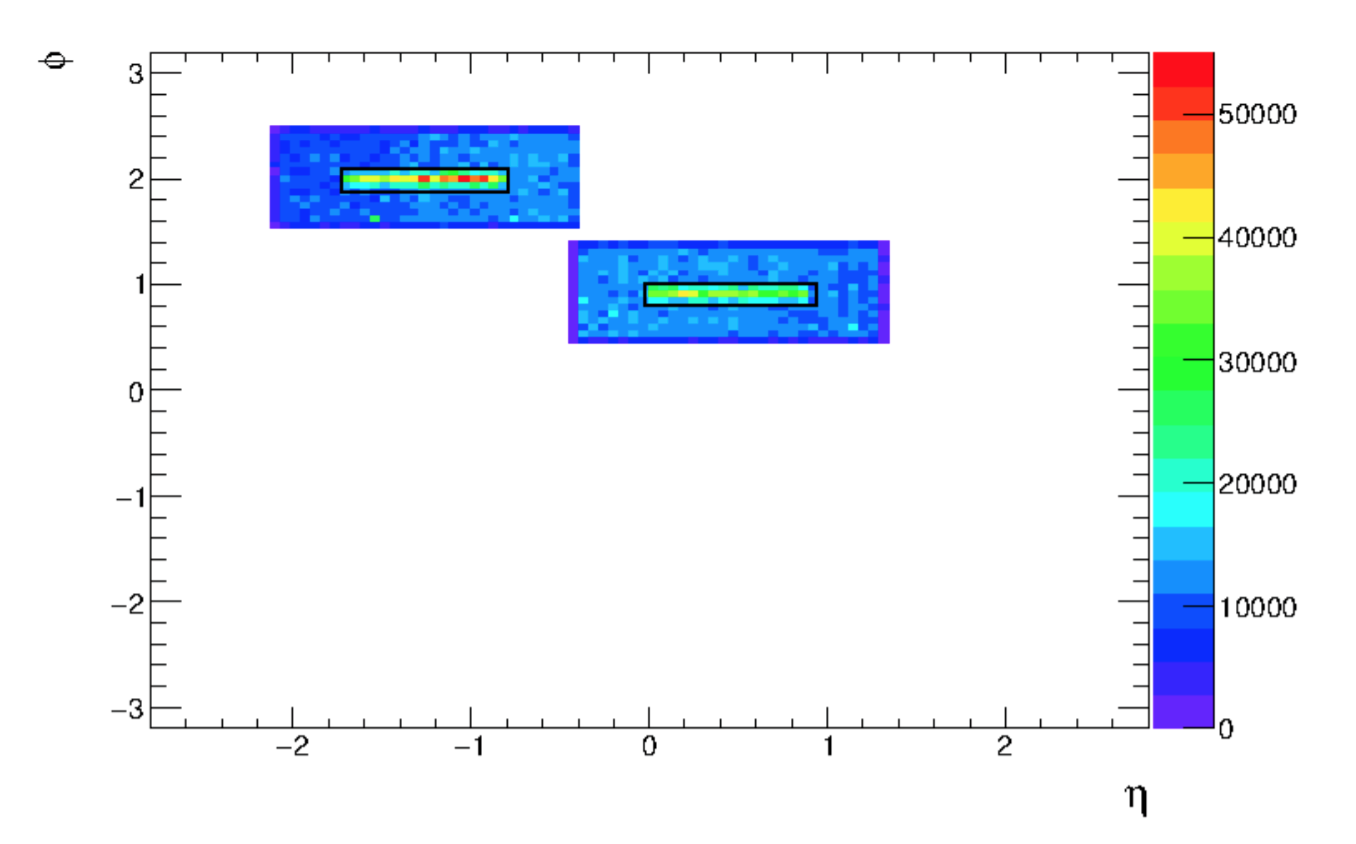
\includegraphics[width=\textwidth]{./Plots/Masked_map.png}
	\caption{$\eta-\phi$-map of small-R jets affected by the masked modules. The inner squares show the regions where the masked modules are.\cite{RodriguezPerez:2126928}}
	\label{masked_modules}
\end{figure}
Jets which are pointing right into the masked modules or close enough to them will be critical miss measured in $p_{\text{T}}$.
This can be especially a source of large $E_{\mathrm{T}}^{\mathrm{miss}}$ and so be critical for processes where large $E_{\mathrm{T}}^{\mathrm{miss}}$ is expected.
As the the modules affect jets in extended regions of $\eta$ and $\phi$, the jet reconstruction will be affected, too.
So it is plausible, that the jets affected by the masked modules will be also miss measured in $\eta$ and $\phi$.

As there are large amounts of $E_{\mathrm{T}}^{\mathrm{miss}}$ in potential monotop events, it is crucial to understand the effects of the masked modules. 
In figure \ref{Phi} are the $\phi$ distributions of the leading large-R jet an $E_{\mathrm{T}}^{\mathrm{miss}}$ are given for monotop data.
\begin{figure}
	\centering
	\begin{subfigure}{0.45\textwidth}
		\includegraphics[width=\textwidth]{./Plots/METphi2_.pdf}
		\caption{Phi distribution of $E_{\mathrm{T}}^{\mathrm{miss}}$ for montotop data.}
	\end{subfigure}
	\begin{subfigure}{0.45\textwidth}
		\includegraphics[width=\textwidth]{./Plots/fatjetphi_.pdf}
		\caption{Phi distribution of leading large-R jets for monotop data.}
	\end{subfigure}
	\caption{}\label{Phi}
\end{figure}
For the $\phi$ distribution of $E_{\mathrm{T}}^{\mathrm{miss}}$ there are two clear peaks positioned right at the position of the masked modules, where the left peak is on the position of LBA10 and the right peak on the position of EBC21.
The peaks in the leading large-R jet $\phi$ distribution are in the opposite $\phi$ direction compared to the $E_{\mathrm{T}}^{\mathrm{miss}}$ $\phi$ distribution. 

\section{JetTileCorrectionTool}
The JetTileCorrectionTool is a Tool which has been developed to correct the effect of masked calorimeter modules on the jet $p_{\text{T}}$ \cite{RodriguezPerez:2126928}.
It supplies the correction by the commonly used technique of inversion of the response function $\mathcal{R}$ \cite{Aad:2014bia}, \cite{LopezMateos:1201006}, \cite{Marshall:1111434}.
The response function is defined as
\begin{equation}
	\mathcal{R}(p_{\text{T}}^{\text{healthy}}) = \frac{p_{\text{T}}^{\text{damaged}}}{p_{\text{T}}^{\text{healthy}}},
\end{equation}
where $p_{\text{T}}^{\text{healthy}}$ and $p_{\text{T}}^{\text{damaged}}$ are generated by MC samples.
The $p_{\text{T}}^{\text{healthy}}$ is created by simulating the ideal detector without masked modules and the $p_{\text{T}}^{\text{damaged}}$ is created by simulating the real detector hence including the masked modules.
Basically for the inversion method
\begin{equation}
\mathcal{R}(p_{\text{T}}^{\text{healthy}}) = \left< \frac{p_{\text{T}}^{\text{damaged}}}{p_{\text{T}}^{\text{healthy}}}\right>
\end{equation}
is calculated.
From that
\begin{equation}
	\mathcal{R}(p_{\text{T}}^{\text{damaged}}) = \frac{p_{\text{T}}^{\text{healthy}}}{p_{\text{T}}^{\text{damaged}}}	
\end{equation}
can be approximated by calculating
\begin{equation}
	p_{\text{T}}^{\text{damaged}} \approx \mathcal{R}(p_{\text{T}}^{\text{healthy}}) p_{\text{T}}^{\text{healthy}}.
\end{equation}
The thus obtained $\mathcal{R}(p_{\text{T}}^{\text{damaged}})$ can be used to correct the reconstructed jet $p_{\text{T}}$ from data by multiplication.
The extent of the correction is calculated depending on the distance of the jet to the masked module.
Currently the correction is only supplied for small-R jets.
Since there is no overlap of the influenced areas for small-R jets, the correction can be separately calculated for the EBC21 and LBA10 module.
The JetTileCorrectionTool decides whether a jet is influenced by the masked modules and categorizes it into three categories:
\begin{itemize}
\item JetTileStatus == 0: Jet is not affected and does not require a correction
\item JetTileStatus == 1: Jet is affected but can be corrected
\item JetTileStatus == 2: Jet is core affected and has to be rejected
\end{itemize}
In the following the JetTileStatus will be abbrevated as TS.
